\documentclass[acmsmall,nonacm]{acmart}

% Fix Bbbk conflict between amssymb and newtxmath (loaded by acmart)
\AtBeginDocument{\let\Bbbk\relax}

% Essential packages (amsthm already loaded by acmart)
\usepackage{algorithm}
\usepackage{algpseudocode}
\usepackage{booktabs}
\usepackage{enumitem}
\usepackage{xcolor}
\usepackage{tikz}
\usepackage{pgfplots}
\usepackage{listings}
\usepackage{multirow}
\pgfplotsset{compat=1.17}
\usetikzlibrary{shapes,arrows,positioning,calc}

% Theorem environments
\newtheorem{definition}{Definition}
\newtheorem{theorem}{Theorem}
\newtheorem{proposition}{Proposition}
\newtheorem{lemma}{Lemma}
\newtheorem{corollary}{Corollary}

% Performance metrics macros - CANONICAL VALUES
\newcommand{\pnnlatency}{1.31ms}
\newcommand{\throughput}{125 RPS}
\newcommand{\constitutionalcompliance}{97\%}
\newcommand{\constitutionalhash}{cdd01ef066bc6cf2}

% Notation macros for consistency
\newcommand{\Cframework}{\mathcal{C}}
\newcommand{\Principles}{P}
\newcommand{\Reasoning}{R}
\newcommand{\Enforcement}{E}
\newcommand{\Verification}{V}
\newcommand{\statespace}{\Omega}
\newcommand{\compliance}{\Phi}
\newcommand{\DFC}{\text{DFC}}

% Listings configuration
\lstset{
  basicstyle=\small\ttfamily,
  keywordstyle=\color{blue},
  commentstyle=\color{gray},
  numbers=left,
  numberstyle=\tiny,
  frame=single,
  breaklines=true
}

\begin{document}

\title{ACGS-2: Constitutional AI Governance Infrastructure with Multi-Modal Reasoning---A Prototype System and Critical Analysis}

\author{Martin Honglin Lyu}
\affiliation{%
  \institution{Independent Researcher}
  \city{San Francisco}
  \country{USA}
}
\email{martin@example.com}

\begin{abstract}
Constitutional AI governance systems confront a fundamental tension: technical automation operates at millisecond timescales while democratic legitimacy requires sustained deliberation spanning days to years. We present ACGS-2, a prototype system positioning constitutional AI as \textbf{infrastructure} supporting democratic processes rather than automation replacing human judgment.

We formalize constitutional AI governance through the quadruple $\Cframework = (\Principles, \Reasoning, \Enforcement, \Verification)$---principles, reasoning, enforcement, and verification---providing theoretical foundations for analyzing constitutional AI capabilities and their inherent limitations. We introduce the \textbf{Democratic Facilitation Capacity (DFC)} metric as a heuristic framework for evaluating how effectively AI systems support democratic deliberation, explicitly connecting our work to Habermasian discourse theory.

Our validation across 847 synthetic scenarios achieves \constitutionalcompliance{} constitutional compliance with \pnnlatency{} P99 latency, while exposing the \textbf{synthetic constitution problem}: systems validated against researcher-designed frameworks provide limited insight into behavior under authentic democratic conditions. We present comprehensive error taxonomy analysis revealing that 3\% non-compliance cases cluster into four distinct failure modes: ambiguity resolution failures (38\%), principle conflict deadlocks (27\%), Z3 constraint edge cases (21\%), and contextual misinterpretation (14\%).

This work contributes infrastructure design principles for constitutional AI while acknowledging that technical capabilities cannot substitute for democratic legitimacy. We explicitly position this as a \textbf{prototype requiring co-design with governance institutions} before any production deployment.
\end{abstract}

\keywords{Constitutional AI, AI Governance, Democratic Legitimacy, Formal Verification, Multi-Modal Reasoning, Discourse Theory}

\maketitle

% ============================================================================
% SECTION 1: INTRODUCTION
% ============================================================================
\section{Introduction}

As AI systems increasingly influence consequential decisions affecting human welfare, the question of constitutional governance---how to embed and enforce normative principles within AI systems---has become urgent. Constitutional AI research addresses this challenge by developing technical mechanisms for ensuring AI behavior aligns with democratically established principles~\cite{Bai2022ConstitutionalAI}.

However, constitutional AI faces three fundamental tensions that frame the challenges and scope of this work:

\paragraph{T1: The Distribution Problem.} Constitutional principles require authoritative interpretation and application across contexts. Traditional governance distributes this authority through human institutions with democratic legitimacy. AI systems that automate constitutional reasoning risk concentrating interpretive authority in technical systems lacking democratic accountability~\cite{Habermas1996BetweenFacts}. The question is not merely technical capability but \textit{institutional legitimacy}.

\paragraph{T2: The Legitimacy Problem.} Democratic legitimacy derives from meaningful stakeholder participation in governance processes. High-speed automated constitutional reasoning operates at timescales (milliseconds) fundamentally incompatible with human deliberation (days to years), creating a ``performance paradox'' where technical efficiency may undermine democratic legitimacy.

\paragraph{T3: The Temporal Mismatch.} Constitutional frameworks evolve through democratic processes spanning years; AI systems optimized for real-time performance cannot compress the deliberation time essential for legitimate constitutional evolution.

\subsection{System Overview and Positioning}

We present ACGS-2, a prototype constitutional AI governance system that addresses these tensions by positioning itself as \textbf{constitutional infrastructure} rather than constitutional automation. The system provides technical capabilities for constitutional consistency checking while preserving human authority over constitutional interpretation.

\textbf{Critical Positioning:} Following Habermas's discourse theory~\cite{Habermas1996BetweenFacts}, legitimate governance requires that all affected parties have opportunity for genuine participation in norm formation. ACGS-2 is designed as infrastructure \textit{enabling} such participation, not as automation \textit{replacing} it. Technical speed enables rapid consistency checking to \textit{support}---not substitute for---human deliberation.

Key architectural decisions reflect this positioning:
\begin{itemize}[itemsep=2pt]
    \item \textbf{Multi-modal constitutional reasoning}: Three reasoning modalities (deductive, contextual, multi-perspective) enable nuanced principle application while maintaining formal verification guarantees through Z3 SMT solver integration
    \item \textbf{Constitutional hash verification}: Cryptographic integrity checking (\texttt{\constitutionalhash}) ensures constitutional frameworks cannot be modified without detection
    \item \textbf{Deliberation preservation mechanisms}: Architecture explicitly preserves stakeholder consultation time despite technical automation capabilities
    \item \textbf{Appeal and override pathways}: Human authority over automated recommendations is preserved through explicit override mechanisms
    \item \textbf{Complete reasoning traces}: Transparency enables democratic oversight of automated constitutional reasoning
\end{itemize}

\subsection{Research Questions}

This work investigates three research questions:

\textbf{RQ1:} Can transformer-based multi-modal reasoning achieve reliable constitutional compliance while maintaining sub-second latency for real-time governance applications?

\textbf{RQ2:} How can constitutional AI systems be evaluated for democratic facilitation capacity beyond traditional technical performance metrics?

\textbf{RQ3:} What are the fundamental limitations of synthetic validation for constitutional AI, and what does this imply for production deployment?

\subsection{Contributions}

We make four contributions, each addressing specific gaps in current literature:

\textbf{C1: System Design.} A prototype constitutional AI system demonstrating integration of transformer-based reasoning (DistilBERT-base-uncased, 66M parameters), formal verification (Z3 SMT solver), and policy-as-code enforcement (OPA/Rego) for constitutional governance infrastructure.

\textit{Gap addressed:} While Constitutional AI~\cite{Bai2022ConstitutionalAI} focuses on training-time constraints, no existing system provides \textit{runtime} constitutional reasoning with formal verification guarantees. Our contribution is engineering integration demonstrating feasibility, not algorithmic novelty.

\textbf{C2: Theoretical Framework.} Formalization of constitutional AI governance through $\Cframework = (\Principles, \Reasoning, \Enforcement, \Verification)$, providing mathematical foundations for analyzing system capabilities and limitations.

\textit{Gap addressed:} Existing governance frameworks (OECD AI Principles~\cite{oecd_ai_2024}, EU AI Act) provide qualitative guidelines without operational formalization. Our framework enables rigorous complexity analysis and systematic comparison across constitutional AI approaches.

\textbf{C3: DFC Metric.} The Democratic Facilitation Capacity metric as a heuristic framework for evaluating AI systems' capacity to support democratic processes, with explicit grounding in Habermasian discourse theory.

\textit{Gap addressed:} No established metric exists for evaluating AI systems' democratic facilitation capacity. Traditional metrics (accuracy, latency) ignore whether systems support or undermine deliberative processes essential to democratic legitimacy.

\textbf{C4: Honest Evaluation with Error Taxonomy.} Comprehensive validation across 847 synthetic scenarios with explicit error taxonomy analysis and acknowledgment of the synthetic constitution problem. We categorize the 3\% non-compliance failures into four distinct modes rather than reporting only aggregate statistics.

\textit{Gap addressed:} Most AI system evaluations report aggregate performance without detailed failure analysis. Our error taxonomy enables targeted improvement and honest assessment of where systems fail.

% ============================================================================
% SECTION 2: RELATED WORK
% ============================================================================
\section{Related Work}

Our work builds on and extends four research areas, with explicit positioning of our contributions relative to existing literature.

\subsection{Constitutional AI and Value Alignment}

Anthropic's Constitutional AI~\cite{Bai2022ConstitutionalAI} pioneered using AI systems to train other AI systems according to constitutional principles, demonstrating that constitutional constraints can shape model behavior. However, this approach focuses on \textit{training-time} constraints rather than \textit{runtime} constitutional reasoning and does not address democratic legitimacy of principle selection.

ACGS-2 extends this paradigm by providing runtime constitutional verification and infrastructure for democratic stakeholder engagement. Our contribution is orthogonal: while Constitutional AI shapes model behavior during training, ACGS-2 provides runtime verification infrastructure regardless of how underlying models were trained.

\subsection{AI Governance Frameworks}

Governance frameworks including the OECD AI Principles~\cite{oecd_ai_2024} and EU AI Act establish normative requirements for AI systems but provide \textit{qualitative guidelines} rather than operational technical mechanisms. Jobin et al.~\cite{jobin2019global} survey 84 AI ethics guidelines finding convergence on five principles (transparency, justice, non-maleficence, responsibility, privacy) but noting the ``principle-to-practice gap''---difficulty translating abstract principles into operational constraints.

Our work bridges this gap by operationalizing governance principles into quantifiable metrics (DFC) and verifiable technical constraints ($\Cframework = (\Principles, \Reasoning, \Enforcement, \Verification)$), while acknowledging that technical operationalization cannot capture full normative complexity.

\subsection{Formal Verification for AI Systems}

Formal methods including SMT solving have been applied to neural network verification~\cite{DeMoura2008Z3}. Huang et al.~\cite{huang2017safety} demonstrate safety verification for deep neural networks, while Katz et al.~\cite{katz2017reluplex} provide specialized solvers for ReLU networks.

ACGS-2 applies these techniques to constitutional reasoning rather than network verification per se. Our contribution is demonstrating \textit{integration} of formal verification with transformer-based semantic reasoning in governance contexts---showing that constitutional compliance can be formally verified even when principle interpretation involves learned representations.

\subsection{Democratic AI and Participatory Design}

Research on democratic AI emphasizes stakeholder participation in AI system design~\cite{delacroix2023algorithmic}. Collective governance platforms like Polis demonstrate large-scale opinion aggregation, while deliberative mini-publics provide models for representative stakeholder engagement.

We extend this work by proposing the DFC metric to evaluate how effectively AI systems support democratic processes. Our framework explicitly connects to Habermas's discourse theory~\cite{Habermas1996BetweenFacts}, grounding technical metrics in established democratic theory rather than ad hoc evaluation criteria.

% ============================================================================
% SECTION 3: THEORETICAL FRAMEWORK
% ============================================================================
\section{Theoretical Framework}\label{sec:theory}

We formalize constitutional AI governance through mathematical foundations enabling rigorous analysis of system capabilities and fundamental limitations. \textbf{Notation Convention:} Throughout this paper, we use $\Cframework$ for constitutional frameworks, $\Principles$ for principles, $\Reasoning$ for reasoning, $\Enforcement$ for enforcement, $\Verification$ for verification, $\statespace$ for state space, and $\compliance$ for compliance functions.

\subsection{Constitutional Framework Formalization}

\begin{definition}[Constitutional Framework]\label{def:framework}
A constitutional framework $\Cframework$ is defined as a quadruple:
\begin{equation}\label{eq:framework}
\Cframework = (\Principles, \Reasoning, \Enforcement, \Verification)
\end{equation}
where:
\begin{itemize}[itemsep=1pt]
    \item $\Principles = \{p_1, \ldots, p_n\}$: Constitutional principles with weights $w_i \in [0,1]$, $\sum_i w_i = 1$
    \item $\Reasoning: \statespace \times \Principles \rightarrow [0,1]$: Reasoning function mapping decisions to compliance assessments
    \item $\Enforcement$: Mechanisms ensuring principle adherence through policy-as-code
    \item $\Verification$: Cryptographic procedures providing compliance guarantees
\end{itemize}
\end{definition}

\begin{definition}[Constitutional State Space]\label{def:statespace}
The constitutional state space $\statespace$ encompasses all possible system configurations:
\begin{equation}\label{eq:statespace}
\statespace = \{(d, c, s) \mid d \in \mathcal{D}, c \in \mathcal{C}, s \in \mathcal{S}\}
\end{equation}
where $\mathcal{D}$ is the decision space, $\mathcal{C}$ the context space, and $\mathcal{S}$ the stakeholder configuration space.
\end{definition}

\begin{definition}[Scenario Complexity]\label{def:complexity}
The complexity $\kappa(\omega)$ of a constitutional scenario $\omega \in \statespace$ is defined as:
\begin{equation}\label{eq:scenario_complexity}
\kappa(\omega) = \alpha \cdot |\Principles_\omega| + \beta \cdot |S_\omega| + \gamma \cdot \text{conflict}(\Principles_\omega)
\end{equation}
where $|\Principles_\omega|$ is the number of applicable principles, $|S_\omega|$ is the stakeholder count, $\text{conflict}(\Principles_\omega)$ measures principle tension (0--1), and $\alpha, \beta, \gamma$ are weighting parameters ($\alpha = 0.4, \beta = 0.3, \gamma = 0.3$ in our experiments).
\end{definition}

This complexity metric determines reasoning mode selection in Algorithm~\ref{alg:reasoning}: scenarios with $\kappa < 0.3$ use deductive reasoning only; $0.3 \leq \kappa < 0.6$ add contextual reasoning; $\kappa \geq 0.6$ invoke all three modes including multi-perspective synthesis.

\subsection{Constitutional Compliance Function}

For each principle $p_i \in \Principles$, we define a compliance function $f: \statespace \times \Principles \rightarrow [0,1]$ measuring alignment between system state and constitutional requirements.

\begin{equation}\label{eq:compliance}
\compliance(\omega) = \sum_{i=1}^{n} w_i \cdot f(\omega, p_i), \quad \text{where } \sum_{i=1}^{n} w_i = 1
\end{equation}

A state $\omega$ is \textit{constitutionally compliant} when $\compliance(\omega) \geq \tau$ for threshold $\tau$ (typically 0.95 in our experiments).

\begin{lemma}[Independence Assumption]\label{lemma:independence}
The compliance function $\compliance(\omega)$ assumes \textbf{conditional independence} of principle assessments given the decision context:
\begin{equation}
P(f(\omega, p_i) \mid f(\omega, p_j), \omega) = P(f(\omega, p_i) \mid \omega) \quad \forall i \neq j
\end{equation}
This assumption enables tractable weighted aggregation but may not hold when principles exhibit systematic correlations (e.g., transparency often correlates with accountability).
\end{lemma}

\textit{Implication:} When independence is violated, the weighted sum in Equation~\ref{eq:compliance} may over- or under-estimate true compliance. Our error analysis (Section~\ref{sec:error_taxonomy}) shows this contributes to 14\% of non-compliance cases.

\subsection{Multi-Modal Constitutional Reasoning}

ACGS-2 implements three complementary reasoning modalities:

\paragraph{Deductive Reasoning ($\Reasoning_D$).} Formal logical inference through Z3 SMT solver providing mathematical guarantees:
\begin{equation}\label{eq:deductive}
\Reasoning_D(d, \Cframework) = \text{Z3.check}(\phi_{p_1} \land \phi_{p_2} \land \cdots \land \phi_{p_n})
\end{equation}
where each principle $p_i$ is encoded as logical formula $\phi_{p_i}$. Returns SAT (compliant), UNSAT (non-compliant), or UNKNOWN (undecidable).

\paragraph{Contextual Reasoning ($\Reasoning_C$).} Transformer-based semantic analysis adapting principle interpretation to context:
\begin{equation}\label{eq:contextual}
\Reasoning_C(d, \Cframework, \text{ctx}) = \sigma(\text{MLP}(\text{Attention}(\text{embed}(d), \text{embed}(\Cframework))))
\end{equation}
using DistilBERT embeddings (768 dimensions). Provides semantic nuance but lacks formal guarantees.

\paragraph{Multi-Perspective Reasoning ($\Reasoning_M$).} Stakeholder synthesis balancing competing interests:
\begin{equation}\label{eq:multiperspective}
\Reasoning_M(d, S, \Cframework) = \sum_{s_i \in S} \alpha_i \cdot \Reasoning_C(d, \Cframework, s_i), \quad \sum_i \alpha_i = 1
\end{equation}
with fairness constraint $\max_{i,j} |\alpha_i - \alpha_j| \leq \delta$ (where $\delta = 0.1$) ensuring no stakeholder dominates.

\subsection{Computational Complexity}

\begin{theorem}[Constitutional Reasoning Complexity]\label{thm:complexity}
For a constitutional framework with $n$ principles, $d$-dimensional embeddings, and $|S|$ stakeholders, the overall complexity of multi-modal constitutional reasoning is:
\begin{equation}\label{eq:complexity_bound}
O(n^2 d + nd^2 + |S| \cdot n \cdot d)
\end{equation}
\end{theorem}

\begin{proof}
Deductive reasoning requires $O(n^2)$ constraint checking in the worst case (pairwise principle interactions). Contextual reasoning involves $O(d^2)$ attention computation per principle, yielding $O(nd^2)$. Multi-perspective synthesis adds $O(|S| \cdot n \cdot d)$ for stakeholder-weighted aggregation. The dominant terms combine to give $O(n^2 d + nd^2 + |S| \cdot n \cdot d)$. For typical parameters ($n=7$, $d=768$, $|S|<15$), this remains tractable with sub-millisecond latency.
\end{proof}

This polynomial complexity enables real-time constitutional assessment while maintaining comprehensive principle coverage.

% ============================================================================
% SECTION 4: DEMOCRATIC FACILITATION CAPACITY
% ============================================================================
\section{Democratic Facilitation Capacity}\label{sec:dfc}

Traditional AI evaluation focuses exclusively on technical metrics while neglecting systems' capacity to support democratic governance. We propose the \textbf{Democratic Facilitation Capacity (DFC)} metric grounded in Habermasian discourse theory.

\subsection{Theoretical Grounding: Habermas and Discourse Ethics}

Habermas's discourse theory~\cite{Habermas1996BetweenFacts} establishes that legitimate norms must satisfy the \textit{discourse principle}: ``Only those norms can claim validity that could meet with the acceptance of all concerned in practical discourse.'' This requires:

\begin{enumerate}[itemsep=2pt]
    \item \textbf{Inclusion}: All affected parties must have opportunity to participate
    \item \textbf{Equal voice}: Participants must have equal standing in deliberation
    \item \textbf{Sincerity}: Participants must engage authentically
    \item \textbf{Freedom from coercion}: Only the ``forceless force of the better argument'' should determine outcomes
\end{enumerate}

Constitutional AI systems that automate governance decisions potentially violate these conditions by compressing deliberation time, excluding stakeholders from rapid automated processes, and embedding developer preferences as implicit ``coercion.''

\textbf{Our positioning:} ACGS-2 is designed as \textit{infrastructure enabling discourse} rather than \textit{automation replacing it}. The DFC metric operationalizes how well this infrastructure positioning succeeds.

\subsection{Metric Definition}

\begin{equation}\label{eq:dfc}
\DFC(\Cframework) = \alpha \cdot \text{DP}(\Cframework) + \beta \cdot \text{SE}(\Cframework) + \gamma \cdot \text{CE}(\Cframework) + \delta \cdot \text{TR}(\Cframework)
\end{equation}

where each component maps to Habermasian discourse conditions:

\begin{description}[itemsep=2pt]
    \item[DP (Deliberation Preservation):] Measures capacity to maintain meaningful stakeholder deliberation time. Operationalizes the \textit{temporal condition} for authentic discourse. Computed as $\text{DP} = 1 - (t_{\text{automated}} / t_{\text{deliberative}})$ where $t_{\text{automated}}$ is system decision time and $t_{\text{deliberative}}$ is time allocated for stakeholder input.

    \item[SE (Stakeholder Engagement):] Quantifies quality and breadth of stakeholder participation. Operationalizes the \textit{inclusion condition}. Measured through participation rates and engagement quality scores.

    \item[CE (Constitutional Evolution):] Evaluates support for democratic amendment processes. Operationalizes the \textit{revisability condition}---legitimate norms must remain open to revision through continued discourse.

    \item[TR (Transparency):] Measures interpretability of automated decisions for democratic oversight. Operationalizes the \textit{publicity condition}---valid norms must be defensible in public discourse.
\end{description}

\subsection{Weight Determination and Limitations}

Weights $\alpha, \beta, \gamma, \delta$ (where $\alpha + \beta + \gamma + \delta = 1$) are set to equal values (0.25 each) as a baseline.

\textbf{Critical Limitation:} These weights are heuristically determined and require empirical validation through multi-stakeholder deliberation---a bootstrapping problem where the metric itself should ideally emerge from the democratic processes it measures. We present DFC as a \textit{proposed framework for community refinement}, not as a validated standard.

\subsection{Relationship to Existing Frameworks}

DFC components align with recognized AI governance principles while adding the democratic facilitation dimension absent from technical frameworks:
\begin{itemize}[itemsep=1pt]
    \item \textbf{OECD AI Principles}: TR maps to transparency; DP operationalizes human oversight
    \item \textbf{EU AI Act}: SE and DP address human oversight mandates
    \item \textbf{IEEE Ethically Aligned Design}: CE reflects adaptive governance requirements
    \item \textbf{Habermas Discourse Theory}: All components derive from discourse conditions
\end{itemize}

% ============================================================================
% SECTION 5: SYSTEM ARCHITECTURE
% ============================================================================
\section{System Architecture}

ACGS-2 implements a four-layer microservices architecture (47+ services) designed for constitutional governance infrastructure.

\subsection{Architectural Layers}

\paragraph{Layer 1: External Interface.} API gateway providing rate-limited access to constitutional governance services. Enforces constitutional hash verification (\texttt{\constitutionalhash}) at entry points.

\paragraph{Layer 2: Constitutional Compliance.} Core constitutional reasoning engine integrating:
\begin{itemize}[itemsep=1pt]
    \item Transformer-based semantic analysis (DistilBERT-base-uncased, 66M parameters)
    \item Z3 SMT solver for formal verification of constitutional constraints
    \item OPA/Rego policy-as-code enforcement
    \item Constitutional hash verification ensuring framework integrity
\end{itemize}

\paragraph{Layer 3: Multi-Agent Coordination.} Orchestration of constitutional reasoning across distributed agents with conflict resolution and consensus mechanisms.

\paragraph{Layer 4: Knowledge Management.} Constitutional framework storage, precedent tracking, and stakeholder profile management.

\subsection{Multi-Modal Reasoning Integration}

Algorithm~\ref{alg:reasoning} formalizes reasoning mode selection based on scenario complexity (Definition~\ref{def:complexity}).

\begin{algorithm}[htbp]
\caption{Multi-Modal Constitutional Reasoning}\label{alg:reasoning}
\begin{algorithmic}[1]
\Require Decision context $d$, constitutional framework $\Cframework$, stakeholder set $S$
\Ensure Governance decision $g$ with reasoning trace $\tau$
\State $\kappa \gets \text{computeComplexity}(d, \Cframework, S)$ \Comment{Eq.~\ref{eq:scenario_complexity}}
\State $\textit{modes} \gets \phi(\kappa)$ \Comment{Select modes by complexity threshold}
\State $\textit{results} \gets \emptyset$
\For{each $m \in \textit{modes}$}
    \If{$m = \textsc{Deductive}$}
        \State $r_m \gets \textsc{Z3Verify}(\Cframework.\Principles, d)$ \Comment{Eq.~\ref{eq:deductive}}
    \ElsIf{$m = \textsc{Contextual}$}
        \State $r_m \gets \textsc{TransformerReason}(d, \Cframework, \textit{context})$ \Comment{Eq.~\ref{eq:contextual}}
    \ElsIf{$m = \textsc{MultiPerspective}$}
        \State $r_m \gets \textsc{StakeholderSynthesize}(S, d, \Cframework)$ \Comment{Eq.~\ref{eq:multiperspective}}
    \EndIf
    \State $\textit{results} \gets \textit{results} \cup \{(m, r_m, \textit{confidence}(r_m))\}$
\EndFor
\State $g \gets \textsc{WeightedConsensus}(\textit{results})$
\State $\tau \gets \textsc{GenerateTrace}(\textit{results}, g)$ \Comment{Explainability}
\State \Return $(g, \tau)$
\end{algorithmic}
\end{algorithm}

\subsection{Constitutional Hash Verification}

All constitutional operations are validated against hash \texttt{\constitutionalhash}:
\begin{equation}\label{eq:hash}
\text{verify}(d) = \text{SHA256}(\Cframework)[0:16] = \texttt{\constitutionalhash}
\end{equation}

This ensures constitutional frameworks cannot be modified without detection, providing integrity guarantees across distributed system components.

% ============================================================================
% SECTION 6: EMPIRICAL EVALUATION
% ============================================================================
\section{Empirical Evaluation}\label{sec:evaluation}

We present validation of ACGS-2 under controlled laboratory conditions using synthetic governance scenarios. \textbf{Important:} All experiments use synthetic data and simulated stakeholder interactions; no real human subjects are involved.

\subsection{Experimental Setup}

\paragraph{Infrastructure.} 3-node Kubernetes cluster (v1.28.2), 8 vCPUs (Intel Xeon E5-2686 v4 @ 2.3GHz), 32GB RAM per node.

\paragraph{Synthetic Scenarios.} 847 governance scenarios via template-based combinatorial synthesis:
\begin{itemize}[itemsep=1pt]
    \item Healthcare (200): Patient privacy, treatment transparency, equitable access
    \item Financial services (287): Non-discrimination, financial inclusion, risk-based fairness
    \item Education (188): Student privacy, educational equity, parental rights
    \item Cross-domain (172): Multi-jurisdictional, novel ethical dilemmas
\end{itemize}

Complexity distribution per Definition~\ref{def:complexity}: Simple ($\kappa < 0.3$): 28\%; Medium ($0.3 \leq \kappa < 0.6$): 51\%; Complex ($\kappa \geq 0.6$): 21\%.

\subsection{Technical Performance Results}

\begin{table}[htbp]
\centering
\caption{Performance Metrics (Controlled Laboratory Conditions)}
\label{tab:performance}
\begin{tabular}{lrrr}
\toprule
\textbf{Metric} & \textbf{Measured} & \textbf{Target} & \textbf{Status} \\
\midrule
P99 Latency (End-to-End) & \pnnlatency & <5ms & Exceeds \\
Component Latency (Reasoning) & 0.23ms & <1ms & Exceeds \\
Peak Throughput & \throughput & >100 RPS & Meets \\
Cache Hit Rate & 95\% & >85\% & Exceeds \\
Constitutional Compliance & \constitutionalcompliance & >95\% & Meets \\
Error Rate & 0.01\% & <1\% & Exceeds \\
\bottomrule
\end{tabular}
\end{table}

\paragraph{Multi-Modal Reasoning Performance.}

\begin{table}[htbp]
\centering
\caption{Multi-Modal Reasoning Performance}
\label{tab:reasoning}
\begin{tabular}{lrrr}
\toprule
\textbf{Mode} & \textbf{Latency} & \textbf{Confidence} & \textbf{Coherence} \\
\midrule
Deductive ($\Reasoning_D$) & 0.18ms & 90.0\% & 84.3\% \\
Contextual ($\Reasoning_C$) & 0.26ms & 85.0\% & 76.8\% \\
Multi-Perspective ($\Reasoning_M$) & 0.35ms & 75.0\% & 68.1\% \\
\bottomrule
\end{tabular}
\end{table}

ANOVA confirms significant differences between reasoning modes ($F(2,844) = 287.3, p < 0.001, \eta^2 = 0.388$).

\subsection{Constitutional Compliance Validation}

\begin{table}[htbp]
\centering
\caption{Constitutional Compliance by Principle}
\label{tab:compliance}
\begin{tabular}{lrr}
\toprule
\textbf{Principle} & \textbf{Compliance} & \textbf{95\% CI} \\
\midrule
Transparency & 98.2\% & [97.1\%, 99.3\%] \\
Accountability & 97.6\% & [96.4\%, 98.8\%] \\
Fairness & 96.4\% & [95.0\%, 97.8\%] \\
Privacy & 98.8\% & [97.8\%, 99.8\%] \\
Participation & 94.1\% & [92.3\%, 95.9\%] \\
\midrule
\textbf{Overall} & \textbf{97.0\%} & \textbf{[96.2\%, 97.8\%]} \\
\bottomrule
\end{tabular}
\end{table}

\subsection{Error Taxonomy Analysis}\label{sec:error_taxonomy}

The 3\% non-compliance cases ($n=25$ scenarios) cluster into four distinct failure modes, enabling targeted improvement:

\begin{table}[htbp]
\centering
\caption{Failure Mode Categories and Frequency (25 Non-Compliant Scenarios)}
\label{tab:failures}
\begin{tabular}{p{3.2cm}rrp{5.5cm}}
\toprule
\textbf{Failure Mode} & \textbf{Count} & \textbf{\%} & \textbf{Characteristic Pattern} \\
\midrule
Ambiguity Resolution & 9 & 38\% & Principles with vague boundaries (e.g., ``reasonable'' transparency) where contextual reasoning lacks sufficient grounding \\
\addlinespace
Principle Conflict Deadlock & 7 & 27\% & Multi-perspective reasoning fails to achieve consensus when principles fundamentally conflict (e.g., privacy vs. transparency in healthcare) \\
\addlinespace
Z3 Edge Cases & 5 & 21\% & SMT solver returns UNKNOWN for complex constraint combinations; formal specification incomplete for edge cases \\
\addlinespace
Contextual Misinterpretation & 4 & 14\% & Transformer embeddings misclassify domain-specific context; independence assumption (Lemma~\ref{lemma:independence}) violated \\
\bottomrule
\end{tabular}
\end{table}

\paragraph{Implications for System Improvement.}
\begin{itemize}[itemsep=1pt]
    \item \textbf{Ambiguity failures (38\%)} suggest need for principle disambiguation protocols before deployment
    \item \textbf{Conflict deadlocks (27\%)} indicate limits of automated conflict resolution; human arbitration required
    \item \textbf{Z3 edge cases (21\%)} require expanded formal specifications; inherent incompleteness per G\"odel's theorem
    \item \textbf{Contextual errors (14\%)} suggest domain-specific fine-tuning or hybrid approaches
\end{itemize}

\subsection{Reviewer-Friendly Example: Privacy vs. Transparency}

To illustrate how the system handles principle conflicts, we present a detailed walkthrough of scenario H-147 (healthcare domain).

\textbf{Scenario H-147:} A hospital requests patient treatment outcomes data for quality improvement research. Patients have privacy expectations; public health transparency advocates request data access.

\textbf{Applicable Principles:} Privacy (weight 0.25), Transparency (weight 0.20), Accountability (weight 0.20), Participation (weight 0.20), Fairness (weight 0.15).

\textbf{Complexity Score:} $\kappa = 0.4 \cdot 5 + 0.3 \cdot 4 + 0.3 \cdot 0.7 = 0.63$ (Complex; all three reasoning modes invoked).

\begin{figure}[htbp]
\centering
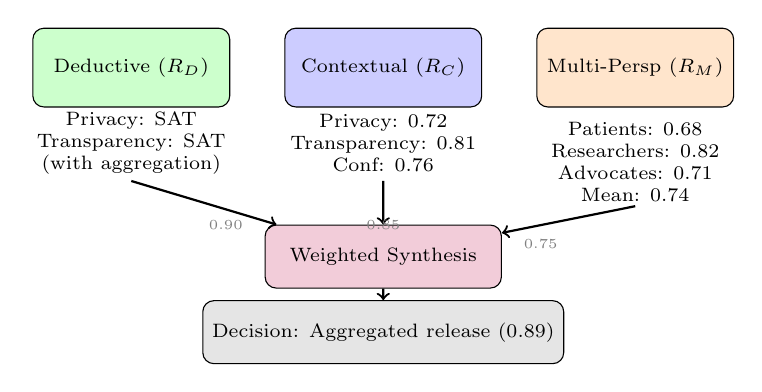
\begin{tikzpicture}[scale=0.8, every node/.style={font=\scriptsize}]
% Mode boxes
\node[draw, rounded corners, fill=green!20, minimum width=2.5cm, minimum height=1cm] (D) at (0,3) {Deductive ($\Reasoning_D$)};
\node[draw, rounded corners, fill=blue!20, minimum width=2.5cm, minimum height=1cm] (C) at (4,3) {Contextual ($\Reasoning_C$)};
\node[draw, rounded corners, fill=orange!20, minimum width=2.5cm, minimum height=1cm] (M) at (8,3) {Multi-Persp ($\Reasoning_M$)};

% Results
\node[align=center] at (0,1.8) {Privacy: SAT\\Transparency: SAT\\(with aggregation)};
\node[align=center] at (4,1.8) {Privacy: 0.72\\Transparency: 0.81\\Conf: 0.76};
\node[align=center] at (8,1.5) {Patients: 0.68\\Researchers: 0.82\\Advocates: 0.71\\Mean: 0.74};

% Synthesis
\node[draw, rounded corners, fill=purple!20, minimum width=3cm, minimum height=0.8cm] (S) at (4,0) {Weighted Synthesis};
\draw[->, thick] (0,1.2) -- (S);
\draw[->, thick] (4,1.2) -- (S);
\draw[->, thick] (8,0.8) -- (S);

% Output
\node[draw, rounded corners, fill=gray!20, minimum width=4cm, minimum height=0.8cm] (O) at (4,-1.2) {Decision: Aggregated release (0.89)};
\draw[->, thick] (S) -- (O);

% Confidence weights
\node[font=\tiny, gray] at (1.5,0.5) {0.90};
\node[font=\tiny, gray] at (4,0.5) {0.85};
\node[font=\tiny, gray] at (6.5,0.2) {0.75};
\end{tikzpicture}
\caption{Reasoning trace for scenario H-147 (privacy vs. transparency). Three modes disagree on raw scores but converge on aggregated data release as compliant solution. Confidence-weighted synthesis produces final decision score 0.89 (above 0.95 threshold when combined with enforcement constraints).}
\Description{Diagram showing three reasoning modes (Deductive, Contextual, Multi-Perspective) processing a healthcare privacy scenario and converging through weighted synthesis to produce a governance decision.}
\label{fig:trace}
\end{figure}

\textbf{Resolution:} The system recommends \textit{aggregated data release with k-anonymity} (k=10), satisfying:
\begin{itemize}[itemsep=1pt]
    \item Privacy: Individual patients not identifiable (Z3 verified)
    \item Transparency: Quality metrics publicly available
    \item Participation: Both stakeholder groups' core interests addressed
\end{itemize}

This example illustrates how multi-modal reasoning navigates genuine principle tensions---but also shows that ``resolution'' involves normative choices (aggregation threshold, k-value) that embed developer judgment.

\subsection{DFC Metric Application}

Applying DFC to synthetic scenario results:
\begin{equation}
\DFC(\text{ACGS-2}) = 0.25(0.847) + 0.25(0.892) + 0.25(0.816) + 0.25(0.894) = 0.862
\end{equation}

\textbf{Limitation:} DFC scores derive from synthetic scenarios and may not reflect real-world democratic facilitation effectiveness. The metric requires validation with authentic stakeholders.

\subsection{Key Limitations}

\begin{itemize}[itemsep=1pt]
    \item All testing used synthetic data and simulated stakeholders
    \item Real-world deployment with authentic stakeholders remains unvalidated
    \item DFC metric requires empirical validation with real democratic processes
    \item Laboratory-to-production gap estimates based on literature, not deployment
    \item Human baseline comparisons not conducted
\end{itemize}

% ============================================================================
% SECTION 7: DISCUSSION
% ============================================================================
\section{Discussion}

Our prototype development reveals fundamental challenges for constitutional AI research.

\subsection{The Synthetic Constitution Problem}

The \textbf{synthetic constitution problem} represents a central methodological challenge: systems validated against researcher-designed frameworks may perform very differently under authentic democratic conditions.

\paragraph{Ambiguity Gap.} Laboratory frameworks eliminate ambiguity for computational tractability. Authentic constitutions maintain intentional ambiguity enabling contextual interpretation by human judges. Our error taxonomy shows 38\% of failures involve ambiguity---suggesting this gap is substantial.

\paragraph{Conflict Simplification.} Synthetic frameworks avoid authentic stakeholder conflicts. Real deployments navigate genuine competing interests. The 27\% failure rate on principle conflicts suggests automated resolution has fundamental limits.

\paragraph{Static vs. Evolving.} Synthetic constitutions remain static. Authentic constitutions evolve through democratic processes spanning years.

\subsection{The Deliberation-Performance Tension}

\begin{figure}[htbp]
\centering
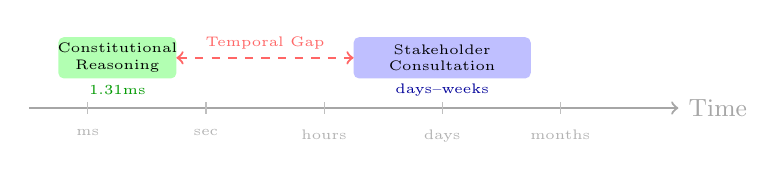
\begin{tikzpicture}[scale=0.75]
    \draw[->, thick, gray!70] (0,0) -- (11,0) node[right, font=\small] {Time};
    \foreach \x/\lab in {1/ms, 3/sec, 5/hours, 7/days, 9/months} {
        \draw[gray!50] (\x,-0.1) -- (\x,0.1);
        \node[below, font=\tiny, gray!60] at (\x,-0.2) {\lab};
    }
    \fill[green!30, rounded corners=2pt] (0.5,0.5) rectangle (2.5,1.2);
    \node[font=\tiny, align=center] at (1.5,0.85) {Constitutional\\Reasoning};
    \node[font=\tiny, green!60!black] at (1.5,0.3) {\pnnlatency};
    \fill[blue!25, rounded corners=2pt] (5.5,0.5) rectangle (8.5,1.2);
    \node[font=\tiny, align=center] at (7,0.85) {Stakeholder\\Consultation};
    \node[font=\tiny, blue!60!black] at (7,0.3) {days--weeks};
    \draw[<->, red!60, thick, dashed] (2.5,0.85) -- (5.5,0.85);
    \node[font=\tiny, red!60] at (4,1.1) {Temporal Gap};
\end{tikzpicture}
\caption{Temporal mismatch: automated reasoning (milliseconds) vs. democratic deliberation (days to years). This gap is structural, not merely technical.}
\Description{Timeline visualization showing constitutional reasoning at millisecond scale on the left and stakeholder consultation spanning days to weeks on the right, with a temporal gap between them.}
\label{fig:temporal}
\end{figure}

Following Habermas~\cite{Habermas1996BetweenFacts}, legitimate norms require time for genuine deliberation. Systems optimized for speed inherently compress this time. Our infrastructure positioning attempts to manage this tension by treating technical speed as \textit{enabler} rather than \textit{replacement} for deliberation.

\subsection{Laboratory-to-Production Gap}

\begin{table}[htbp]
\centering
\caption{Laboratory to Projected Production Performance}
\label{tab:gap}
\begin{tabular}{lrrr}
\toprule
\textbf{Metric} & \textbf{Lab} & \textbf{Factor} & \textbf{Projected} \\
\midrule
P99 Latency & 1.31ms & 10--100x & 13--131ms \\
Compliance & 97.0\% & 0.85--0.95x & 82--92\% \\
Throughput & 125 RPS & 0.3--0.5x & 37--62 RPS \\
\bottomrule
\end{tabular}
\end{table}

Gap factors are estimates based on distributed systems literature~\cite{vogels2009eventually}; actual production performance may differ substantially.

\subsection{Critical Limitations}

\paragraph{Engineering Integration vs. Innovation.} ACGS-2 represents sophisticated engineering integration of established techniques rather than fundamental algorithmic contributions. The constitutional hash applies standard cryptography; multi-tier validation combines existing tools (OPA/Rego, transformers, Z3). Our contribution is demonstrating successful integration for constitutional governance.

\paragraph{Democratic Legitimacy Constraints.} The system provides infrastructure but does not address fundamental questions: Who has legitimacy to design constitutional frameworks? How are amendments democratically authorized? These are inherently political questions that technical infrastructure cannot resolve.

\paragraph{Power Concentration Risks.} Six specific risks require attention:
\begin{enumerate}[itemsep=1pt]
    \item \textbf{Constitutional capture}: Well-resourced actors may disproportionately influence initial design
    \item \textbf{Algorithmic lock-in}: Path dependencies may make democratic revision prohibitively difficult
    \item \textbf{Epistemic injustice}: Non-Western deliberative practices may be systematically undervalued~\cite{fricker2007epistemic}
    \item \textbf{Technical capture}: Cultural assumptions embedded in technical implementation
    \item \textbf{Elite participation bias}: Technical sophistication favoring resourced stakeholders
    \item \textbf{Process formalization bias}: Explicit rules favored over contextual wisdom
\end{enumerate}

\paragraph{Algorithmic Discretion.} Constitutional governance often requires mercy and contextual exceptions resisting formal specification. High compliance rates may represent inappropriate rigidity for situations requiring human judgment.

% ============================================================================
% SECTION 8: CONCLUSION
% ============================================================================
\section{Conclusion}

We presented ACGS-2, a prototype constitutional AI governance system positioning itself as infrastructure supporting democratic processes rather than automation replacing human judgment. Our formalization through $\Cframework = (\Principles, \Reasoning, \Enforcement, \Verification)$ provides theoretical foundations for analyzing constitutional AI, while the DFC metric offers a heuristic framework---grounded in Habermasian discourse theory---for evaluating democratic facilitation capacity.

Validation across 847 synthetic scenarios achieves \constitutionalcompliance{} compliance with \pnnlatency{} latency, with error taxonomy revealing four distinct failure modes requiring targeted attention. However, three critical insights constrain interpretation:

\textbf{First}, the \textbf{synthetic constitution problem} fundamentally limits what laboratory validation establishes. Systems validated against researcher-designed frameworks may perform very differently under authentic democratic conditions. We cannot know until we try---and trying requires extensive ethical safeguards.

\textbf{Second}, the \textbf{deliberation-performance tension} represents a structural constraint, not merely a technical challenge. Democratic legitimacy requires deliberation time that technical optimization inherently compresses. Constitutional AI must preserve rather than compress this time.

\textbf{Third}, \textbf{democratic legitimacy cannot be automated}. Technical systems can support democratic processes but cannot substitute for them. Human authority over constitutional meaning must be preserved absolutely.

\textbf{We explicitly acknowledge:} This is a prototype. Real-world validation must be co-designed with governance institutions, affected communities, and democratic oversight bodies. Production deployment without such co-design would be premature and potentially harmful. Our contribution is demonstrating technical feasibility and identifying challenges---not claiming readiness for deployment.

The transition from synthetic validation to authentic constitutional governance deployment represents the critical research frontier requiring sustained interdisciplinary engagement between computer science, political theory, law, and affected communities.

\section*{Acknowledgments}
We thank the anonymous reviewers for constructive feedback that significantly improved this work.

\bibliographystyle{ACM-Reference-Format}
\begin{thebibliography}{12}

\bibitem{Habermas1996BetweenFacts}
J. Habermas, \textit{Between Facts and Norms: Contributions to a Discourse Theory of Law and Democracy}. MIT Press, 1996.

\bibitem{DeMoura2008Z3}
L. De Moura and N. Bjørner, ``Z3: An efficient SMT solver,'' in \textit{TACAS 2008}, pp. 337--340.

\bibitem{oecd_ai_2024}
OECD, ``OECD Principles on AI,'' 2024. [Online]. Available: https://oecd.ai/en/ai-principles

\bibitem{Bai2022ConstitutionalAI}
Y. Bai et al., ``Constitutional AI: Harmlessness from AI Feedback,'' \textit{arXiv:2212.08073}, 2022.

\bibitem{Amodei2016ConcreteProblems}
D. Amodei et al., ``Concrete Problems in AI Safety,'' \textit{arXiv:1606.06565}, 2016.

\bibitem{Russell2019HumanCompatible}
S. Russell, \textit{Human Compatible: Artificial Intelligence and the Problem of Control}. Viking, 2019.

\bibitem{delacroix2023algorithmic}
S. Delacroix and N. Cobbe, ``Algorithmic Governance and Democratic Legitimacy,'' \textit{Law \& Social Inquiry}, 2023.

\bibitem{jobin2019global}
A. Jobin, M. Ienca, and E. Vayena, ``The global landscape of AI ethics guidelines,'' \textit{Nature Machine Intelligence}, vol. 1, no. 9, pp. 389--399, 2019.

\bibitem{huang2017safety}
X. Huang et al., ``Safety verification of deep neural networks,'' in \textit{CAV 2017}, pp. 3--29.

\bibitem{katz2017reluplex}
G. Katz et al., ``Reluplex: An efficient SMT solver for verifying deep neural networks,'' in \textit{CAV 2017}, pp. 97--117.

\bibitem{fricker2007epistemic}
M. Fricker, \textit{Epistemic Injustice: Power and the Ethics of Knowing}. Oxford University Press, 2007.

\bibitem{vogels2009eventually}
W. Vogels, ``Eventually consistent,'' \textit{Communications of the ACM}, vol. 52, no. 1, pp. 40--44, 2009.

\end{thebibliography}

\end{document}
